\documentclass[final,5p,times,twocolumn]{elsarticle}

\usepackage{lmodern}
\usepackage[T1]{fontenc}

\usepackage{amsmath,amssymb,amsfonts}
\usepackage{graphicx}
\usepackage{tikz}
\usetikzlibrary{arrows.meta,positioning,calc}
\definecolor{hiblue}{HTML}{0072B2}   % the palette of fig2.pdf
\definecolor{hired}{HTML}{D55E00}
\definecolor{higreen}{HTML}{009E73}
\usepackage{lineno}
\usepackage{array}         % >{\raggedright} column prefixes, so a
                           % narrow table column breaks instead of
                           % overfilling
\newcolumntype{R}[1]{>{\raggedright\arraybackslash}p{#1\textwidth}}
\usepackage{url}           % elsarticle loads neither url nor
                           % hyperref; \url breaks the repository
                           % address, \texttt would overfull it

\tolerance=1500
\emergencystretch=2em
\hyphenpenalty=100
\hbadness=4000

\newcommand{\R}{\mathbb{R}}
\newcommand{\E}{\mathbb{E}}
\newcommand{\dvec}{\mathbf{d}}
\newcommand{\dhat}{\hat{\mathbf{d}}}
\newcommand{\Var}{\mathrm{Var}}
\newcommand{\Std}{\mathrm{Std}}
\newcommand{\lloss}{\ell}

\journal{Reliability Engineering \& System Safety}

\begin{document}

\begin{frontmatter}

\title{Information loss of fixed linear health indicators under competing
degradation mechanisms and variable operating conditions}

\author[a]{Huy Hoang Le}
\ead{lhhoang@powermore.vn}
\author[b]{Kim-Anh Nguyen\corref{cor}}
\ead{nkanh@dut.udn.vn}
\cortext[cor]{Corresponding author}
\affiliation[a]{organization={R\&D Department, PowerMore Ltd.},
  city={Da Nang}, postcode={550000}, country={Viet Nam}}
\affiliation[b]{organization={Faculty of Electrical Engineering, University
  of Science and Technology, The University of Danang},
  city={Da Nang}, postcode={550000}, country={Viet Nam}}

\begin{abstract}
Predictive maintenance often estimates remaining useful life from a health
indicator: a fixed-weight combination of condition-monitoring signals. When a
component degrades through several mechanisms at different rates, the
combination most informative about remaining life, the informative
direction, changes with age, and no fixed indicator can follow it. This
paper quantifies the information such an indicator loses and whether the
operating point, which sets those rates, can reduce it. For units differing
only in age, the loss depends on one angle between the indicator and the
informative direction and fixes the increase in the error variance of the
remaining-life estimate. If that direction turns through an arc $\Phi$ over
life, a well-placed fixed indicator increases the variance by at most a
factor $1/\cos^{2}(\Phi/2)$. On $129$ lithium-ion cells the arc is $30.7^{\circ}$,
so by at most $7.5\%$, and remaining-life estimates and replacement decisions
are as good with a fixed indicator as with all signals. In simulation,
adjusting the operating point reduces this already small loss $47$-fold but
barely improves the estimate, while lifetime varies $19$-fold. Unless the arc
is large, a fixed indicator is adequate and the operating point is better
chosen for lifetime.
\end{abstract}

\begin{keyword}
health indicator \sep remaining useful life \sep prognostics \sep
predictive maintenance \sep competing degradation mechanisms \sep
operating conditions \sep information loss
\end{keyword}

\end{frontmatter}

\linenumbers

\section{Introduction}
\label{sec:intro}

Predictive maintenance replaces or repairs a component shortly before it is
expected to fail, rather than on a fixed schedule or after failure. The
expectation comes from an estimate of the component's remaining useful life,
and that estimate is in turn computed from condition monitoring. Monitoring
seldom passes its raw measurements to the estimation algorithm: channels such
as vibration, temperature, impedance and capacity are first combined into a
single number, the health indicator, and the algorithm sees only that
number~\cite{lei2018,coble2009}. In practice the weights of the combination
are usually fixed when the monitoring system is designed, because they are
embedded in firmware, frozen by certification, or impractical to re-tune in
the field. The indicator therefore determines how accurately the remaining
useful life can be estimated and, through that estimate, how early
maintenance must be scheduled to keep the risk of failure acceptable.

A fixed weighting is not always a good weighting. Engineering components
commonly degrade through several mechanisms at once, and these mechanisms
need not progress at the same rate. In a lithium-ion cell, for example,
capacity fade and the growth of internal resistance arise from different
physical processes and need not evolve in proportion; one mechanism may
dominate early in life while another accelerates towards failure. It helps
to picture the monitoring channels as the axes of a space. As the component
ages, its readings move through this space, and the direction in which they
move is the combination of channels that changes most with age, and hence
the one that says most about the remaining life. When the mechanisms progress
at different rates, this direction turns as the component ages. A fixed
indicator is a fixed direction in the same space, so it can be aligned with
the most informative combination at one moment only, and the information it
discards at other moments cannot be recovered by any prognostic algorithm
that uses the indicator~\cite{le2026jestech}.

Two practical questions follow. The first is how much information a fixed
indicator actually loses, and whether this can be assessed before the
indicator is designed, when a different weighting or an adaptive indicator
can still be chosen. The second concerns the operating conditions, such as
temperature, load or duty cycle. These vary, either because the duty imposes
them or because the operator selects them, and in both cases they change the
relative rates of the mechanisms and hence the direction in which the
readings move. Operators already select operating points to extend
life~\cite{hac2020,rulcontrol2025,salazar2017system}; the question is
whether the operating point could also be chosen to keep a fixed indicator
aligned, and whether doing so would be worthwhile.

Existing work addresses the first question from the perspective of indicator
construction, with criteria that differ from the one used here. Health
indicators are constructed from data so that they change steadily and
predictably with age, as measured by criteria such as monotonicity and
trendability~\cite{coble2009,wen2021generalized}, or by fusing sensors into a
composite index whose weights are fitted once, for example so that the fused
index has a consistent value at failure or follows a prescribed degradation
model~\cite{liu2013fusion,song2018fusion,fang2017multistream,wang2022building,li2025dualpurpose};
such indices have also been built under several operating
conditions~\cite{yan2016multiple} and learned by neural
networks~\cite{guo2017}, and reviews survey the resulting
pipelines~\cite{lei2018,javed2017}. Once fitted, these indices are fixed and
linear in the channels, which is precisely the class of indicators considered
in this paper, but none of the construction criteria measures how much
information about remaining life the index discards as the mechanisms
diverge. State-space fusion~\cite{li2021remaining} avoids a fixed weighting
but tracks a single degradation state, in which case the direction cannot
turn. Section~\ref{sec:cells} compares one fusion criterion with the design
proposed here on measured cells.

The second question connects to degradation modelling and to operation.
Degradation under time-varying operating conditions is well
modelled~\cite{meeker1998,ye2015,si2011,zhang2018,bian2015degradation,li2019remaining,jahani2021stochastic},
and several degradation characteristics are known to respond differently to
the same environment~\cite{lin2025modeling} or to depend on one
another~\cite{chen2026causal}. A separate body of work selects the operating
point, or the load or production rate it implies, to extend life or to
balance performance against
reliability~\cite{hac2020,rulcontrol2025,salazar2017system,langeron2015modeling,uithetbroek2021joint,zuo2024deterioration},
and prognostic accuracy has been assessed through its consequences for
predictive maintenance~\cite{kamariotis2024metric}. These studies treat the
monitoring signal as given; none asks what the operating point does to the
information a fixed indicator retains. Our previous work bounded the
information that any fixed compression of the channels retains along a
single, given degradation trajectory~\cite{le2026jestech}, and the number of
run-to-failure units required to learn such a compression~\cite{le2026mst}.
The present paper builds on that analysis: it expresses the loss of a single
linear indicator through one angle, relates the loss to the error of the
remaining-life estimate and to maintenance decisions, bounds it by how far
the informative direction turns, tests the bound on measured data, and lets
the trajectory change with the operating point.

The main contributions of this paper are as follows.
\begin{itemize}
\item The information discarded by a fixed linear indicator is shown to be an
exact function of a single misalignment angle, and the resulting inflation of
the error variance of the remaining-life estimate, and of the safety margin
of a predictive replacement policy, is obtained in closed form
(Section~\ref{sec:model}).
\item The arc traversed by the informative direction over the service life
is shown to bound this inflation before any indicator is designed, which
yields a five-step design procedure that requires run-to-failure data only
(Section~\ref{sec:arc}).
\item In a case study on measured battery cells the bound is $7.5\%$, which
corresponds to a safety margin of a predictive replacement policy at most
$3.7\%$ wider; a leave-one-out remaining-life estimator and a replacement
policy using the fixed indicator perform as well as ones using all channels
(Section~\ref{sec:cells}).
\item Selecting the operating point to keep the indicator aligned reduces the
information loss substantially but leaves the error of a practical
remaining-life estimator essentially unchanged, whereas the operating point
alters the lifetime by an order of magnitude (Section~\ref{sec:steer}).
Public run-to-failure data support the premise that the informative
direction turns but do not permit a test of the effect of the operating
point on degradation (Section~\ref{sec:data}).
\end{itemize}

The remainder of the paper proceeds from the general to the specific.
Section~\ref{sec:model} states the degradation model, defines the
information loss and lists the assumptions. Section~\ref{sec:arc} bounds the
loss by how far the informative direction turns and derives the design
procedure that follows from the bound. Section~\ref{sec:cells} applies the
procedure to measured lithium-ion cells, up to a maintenance decision.
Section~\ref{sec:steer} examines, on a synthetic system, whether selecting
the operating point is worthwhile, and Section~\ref{sec:data} examines the
assumptions on public run-to-failure data. Section~\ref{sec:discussion}
answers the two questions and discusses the implications. Derivations are
given in \ref{app:derivations}.

\section{Problem formulation}
\label{sec:model}

This section states how the mechanisms degrade and how they are observed
(Sections~\ref{sec:degmodel} and~\ref{sec:direction}), defines the
information that a fixed indicator loses and relates it to the error of the
remaining-life estimate (Section~\ref{sec:loss}), and closes with the
assumptions on which the rest of the paper rests.
Figure~\ref{fig:framework} gives an overview of the construction.

\begin{figure*}[tb]
\centering
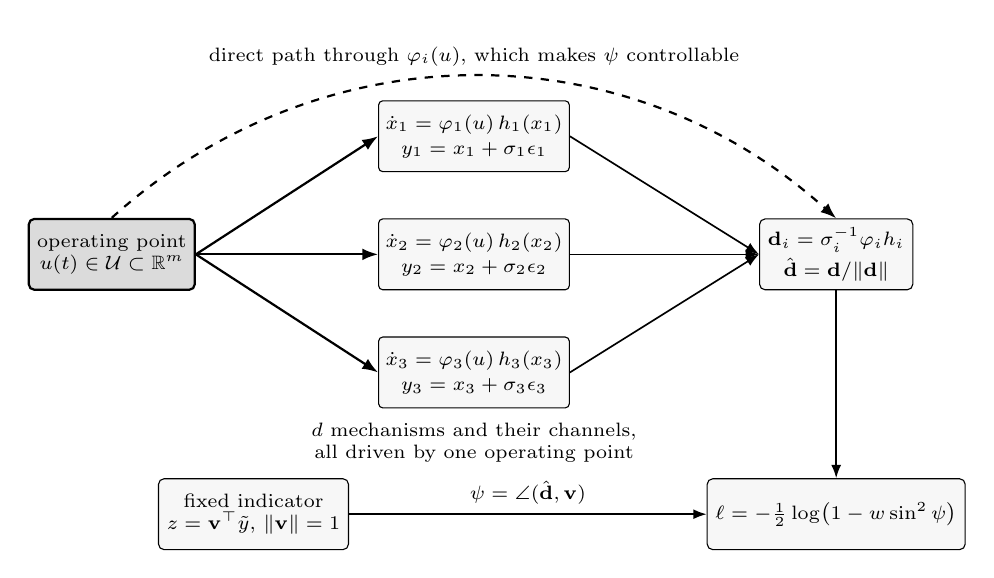
\begin{tikzpicture}[
  font=\small,
  b/.style={draw, rounded corners=1.5pt, align=center, inner sep=2.5pt,
            minimum height=9mm, fill=black!3, font=\scriptsize},
  lev/.style={draw, rounded corners=2pt, align=center, inner sep=3pt,
              minimum height=9mm, fill=black!14, thick, font=\scriptsize},
  ob/.style={draw, rounded corners=2pt, align=center, inner sep=3pt,
             minimum height=9mm, fill=black!3, font=\scriptsize},
  a/.style={-{Latex[length=1.7mm]}, semithick},
  th/.style={-{Latex[length=2mm]}, thick},
  lbl/.style={font=\scriptsize, inner sep=1pt}]

\node[lev] (u) at (0,0) {operating point\\$u(t)\in\mathcal U\subset\R^{m}$};

\foreach \i/\y in {1/15mm, 2/0mm, 3/-15mm} {
  \node[b] (m\i) at (46mm,\y)
        {$\dot x_{\i}=\varphi_{\i}(u)\,h_{\i}(x_{\i})$\\[1pt]
         $y_{\i}=x_{\i}+\sigma_{\i}\epsilon_{\i}$};
}
\foreach \i in {1,2,3} { \draw[th] (u.east) -- (m\i.west); }

\node[lbl, anchor=north, align=center] at (46mm,-21mm)
      {$d$ mechanisms and their channels,\\ all driven by one operating point};

\node[ob] (d) at (92mm,0)
      {$\dvec_i=\sigma_i^{-1}\varphi_i h_i$\\[1pt]$\dhat=\dvec/\|\dvec\|$};
\foreach \i in {1,2,3} { \draw[a] (m\i.east) -- (d.west); }

\node[ob] (v) at (18mm,-33mm)
      {fixed indicator\\$z=\mathbf v^{\top}\tilde y$, $\|\mathbf v\|=1$};
\node[ob] (l) at (92mm,-33mm)
      {$\lloss=-\tfrac12\log\!\big(1-w\sin^{2}\psi\big)$};

\draw[a] (d) -- (l);
\draw[a] (v) -- node[above, font=\scriptsize]
      {$\psi=\angle(\dhat,\mathbf v)$} (l);

\draw[th, dashed] (u.north) to[out=42, in=138]
      node[above, font=\scriptsize]
      {direct path through $\varphi_i(u)$, which makes $\psi$ controllable}
      (d.north);
\end{tikzpicture}
\caption{Overview of the problem formulation. One operating point drives all $d$ mechanisms, each observed through its own channel. The informative direction $\dhat$ is the weighting of the whitened channels that responds most strongly to the remaining life; the loss $\lloss$ of a fixed indicator $\mathbf v$ depends only on the angle $\psi$ between them. The operating point affects $\dhat$ both through the damage and directly through the stress factors $\varphi_i(u)$; the direct path makes $\psi$ controllable.}
\label{fig:framework}
\end{figure*}

\subsection{Degradation model with operating-point dependence}
\label{sec:degmodel}

A component degrades through $d$ mechanisms, with damage states
$x=(x_1,\dots,x_d)$, $x_i\ge0$. A single operating point
$u(t)\in\mathcal U\subset\R^{m}$, comprising $m$ adjustable variables such as
temperature, load and duty cycle, drives all of them; the envelope
$\mathcal U$ is the bounded range of operating points allowed in service.
The damage of each mechanism grows at a rate that depends on the operating
point and on the damage already accumulated:
\begin{equation}
\dot x_i=\varphi_i(u)\,h_i(x_i),\qquad i=1,\dots,d.
\label{eq:plant}
\end{equation}
The stress factor $\varphi_i(u)>0$ expresses how much faster mechanism $i$
runs at $u$ than at a reference operating point, and the shape function
$h_i(x_i)>0$ describes how its rate changes as damage accumulates. The two
effects enter as separate factors, which makes the model separable. This is
the standard accelerated-life form~\cite{meeker1998}: in the Arrhenius model
$\varphi_i(u)=A_i\exp(-E_i/(kT))$, with activation energy $E_i$, absolute
temperature $T$ and Boltzmann constant $k$, and suitable choices of $h_i$
yield exponential, power-law and stretched-exponential
degradation~\cite{le2026jestech}. Damage is normalised such that each
mechanism exhausts the component at unity, and the component is withdrawn
from service when the first mechanism reaches a condemnation limit
$x_f\in(0,1]$:
\begin{equation}
T_f=\inf\{t\ge0:\textstyle\max_i x_i(t)\ge x_f\}.
\label{eq:tf}
\end{equation}
The lifetime $T_f$ depends on the operating point, and the normalised life
$\tau=t/T_f$ runs from $0$ at the start of service to $1$ at withdrawal.

\subsection{Remaining useful life and the informative direction}
\label{sec:direction}

The quantity to be estimated is the remaining useful life $R(t)=T_f-t$. For
a single unit with known parameters, \eqref{eq:plant} would determine it
exactly; the uncertainty arises because the units of a fleet
differ~\cite{meeker1998}. The analysis assumes that they differ only in age:
all units follow a common degradation path, and each is at a different
position along it, as are identical components installed at different
times. Such a population is called a time-shift population
(Fig.~\ref{fig:lossmech}(a)), and $R$ is taken
to be Gaussian over it with variance $\Var[R]$. For two units of such a
population whose remaining lives differ slightly, the damage states differ,
to first order, only along the direction in which the damage is currently
growing. Since $R$ decreases at unit rate, the sensitivity of mechanism $i$
to the remaining life is therefore
\begin{equation}
\frac{\partial x_i}{\partial R}=-\frac{\partial x_i}{\partial t}
=-\varphi_i(u)\,h_i(x_i).
\label{eq:sens}
\end{equation}

Each mechanism is observed through a dedicated channel,
\begin{equation}
y_i=x_i+\sigma_i\epsilon_i,\qquad i=1,\dots,d,
\label{eq:obs}
\end{equation}
with independent standard normal noise $\epsilon_i$ and noise level
$\sigma_i$. This pairing of channels with mechanisms is an assumption:
condition monitoring in general yields $y=H(x,u)+\epsilon$, with sensors that
mix mechanisms, and Section~\ref{sec:data} shows that raw turbofan sensors
violate it. To make channels with different units and noise levels
comparable, each is divided by its noise level, which is called whitening;
the whitened readings $\tilde y=(y_i/\sigma_i)$ at one inspection are called
the record. By \eqref{eq:sens}, the record responds to the remaining life
through the signal vector
\begin{equation}
\dvec=\big[\sigma_i^{-1}\varphi_i(u)h_i(x_i)\big]_{i=1}^{d},\qquad
\dhat=\dvec/\|\dvec\|.
\label{eq:dvec}
\end{equation}
The norm $\|\dvec\|$ measures how strongly the record responds to the
remaining life, and the unit vector $\dhat$, a point on the unit sphere of
the $d$-dimensional space of whitened channels, is the combination of
channels along which it responds. It is referred to as the
\emph{informative direction}: the weighting of the channels that, at the
current state, carries the most information about the remaining life. All
entries of $\dvec$ are positive, and $\dhat$ depends on both the state and
the operating point. The operating point affects $\dhat$ through two paths:
indirectly, through the damage it produces, and directly, through
$\varphi_i(u)$.

\subsection{Information loss of a fixed linear indicator}
\label{sec:loss}

A fixed linear indicator combines the record with a weight vector selected
once at the design stage:
\begin{equation}
z=\mathbf v^{\top}\tilde y,\qquad \|\mathbf v\|=1 .
\label{eq:hi}
\end{equation}
The weight vector is a second point on the same unit sphere. An indicator
defined on raw measurements, with weights $\mathbf a$, is the same mapping
with $\mathbf v\propto\Sigma^{1/2}\mathbf a$, where
$\Sigma=\mathrm{diag}(\sigma_i^{2})$. Let $\psi$ denote the angle between
$\mathbf v$ and $\dhat$, called the misalignment, and let
$\gamma=\|\dvec\|^{2}\Var[R]$ denote the signal-to-noise ratio of the
record, that is, the spread of the remaining life across the population as
seen through the record, relative to the noise. Linearising the record about
the nominal path renders it jointly Gaussian with $R$; the indicator then
retains the fraction $\cos^{2}\psi$ of the signal and all of the noise
(Fig.~\ref{fig:lossmech}(b)).

Information is measured here by the mutual information between the
remaining life and the observation, in natural units (nats), and the loss
$\lloss$ is the information about $R$ carried by the record but not by the
indicator. It is therefore (\ref{app:loss})
\begin{equation}
\lloss=\tfrac12\log\frac{1+\gamma}{1+\gamma\cos^{2}\psi}
=-\tfrac12\log\!\big(1-w\sin^{2}\psi\big),
\label{eq:exact}
\end{equation}
with $w=\gamma/(1+\gamma)$. The loss has a direct statistical meaning: the
error variance of the optimal estimate of $R$ based on the indicator exceeds
that based on the record by the factor
\begin{equation}
\frac{\Var[R\mid z]}{\Var[R\mid\tilde y]}=\frac{1+\gamma}{1+\gamma\cos^{2}\psi}
=e^{2\lloss}.
\label{eq:mmse}
\end{equation}
A loss of $0.01$~nat, for instance, means an error variance about $2\%$
larger than with all channels, and this excess, $e^{2\lloss}-1$, is the
quantity that the rest of the paper reports alongside the loss. The loss
depends on the indicator only through the single angle $\psi$, and for small
misalignment $\lloss\approx\tfrac{w}{2}\psi^{2}$. The design objective is
its average over the service life,
\begin{equation}
\bar\lloss=\frac{1}{T_f}\int_{0}^{T_f}\lloss(t)\,dt .
\label{eq:objective}
\end{equation}
The same reduction applies when the indicator is read at many inspections,
with $\gamma$ summed over the records of the inspections and
$\sin^{2}\psi$ averaged with weights $\|\dvec\|^{2}$ (Supplementary
Section~S2).

The loss also bears directly on maintenance decisions. Under the Gaussian
model, a predictive replacement policy that replaces a unit once its
probability of failing within a lead time $t_{\mathrm{lead}}$ reaches
$\alpha$ does so when the estimated remaining life falls to
$t_{\mathrm{lead}}+\zeta_{\alpha}s_R$, where $s_R$ is the standard deviation
of the remaining life given the observation and $\zeta_{\alpha}$ the standard
normal quantile of order $1-\alpha$. The safety margin $\zeta_{\alpha}s_R$ is,
on average, remaining life discarded at replacement beyond the lead time, and
a fixed indicator multiplies it by $e^{\lloss}$ relative to the record
(Fig.~\ref{fig:lossmech}(c)).
Decision-oriented assessments of prognostic algorithms weigh precisely this
margin against the risk of failure~\cite{kamariotis2024metric}.

%<mechfig:loss> generated by make_mechfigs.py -- edit there, not here
\begin{figure*}[tb]
\centering
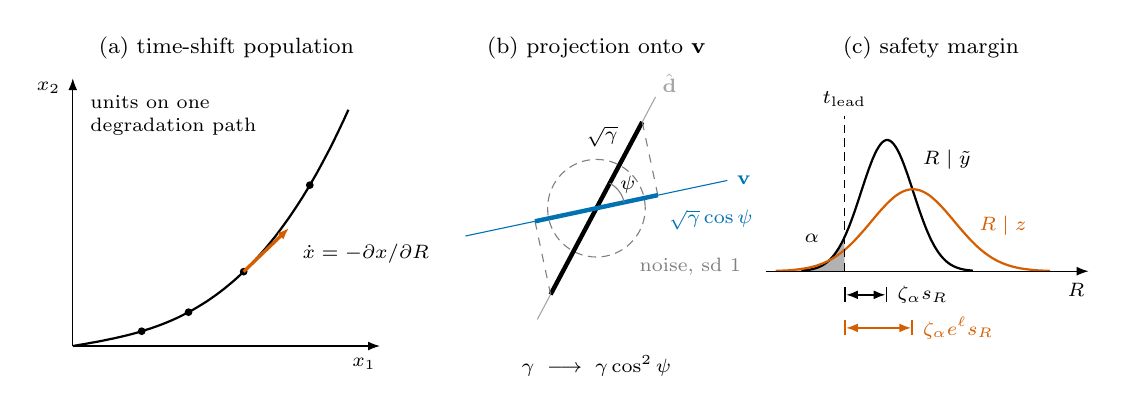
\begin{tikzpicture}[font=\scriptsize, >={Latex[length=1.5mm]},
  ttl/.style={font=\footnotesize, anchor=north}]
% (a) time-shift population in damage space
\node[ttl] at (1.95,4.05) {(a) time-shift population};
\draw[->] (0,0) -- (3.9,0) node[below left=1pt and -2pt] {$x_1$};
\draw[->] (0,0) -- (0,3.4) node[below left=-2pt and 1pt] {$x_2$};
\draw[thick] plot coordinates {(0,0) (0.058,0.01) (0.117,0.02) (0.175,0.03) (0.233,0.041) (0.292,0.051) (0.35,0.062) (0.408,0.074) (0.467,0.086) (0.525,0.098) (0.583,0.111) (0.642,0.125) (0.7,0.139) (0.758,0.154) (0.817,0.17) (0.875,0.188) (0.933,0.206) (0.992,0.225) (1.05,0.245) (1.108,0.266) (1.167,0.289) (1.225,0.313) (1.283,0.338) (1.342,0.365) (1.4,0.394) (1.458,0.424) (1.517,0.455) (1.575,0.489) (1.633,0.524) (1.692,0.561) (1.75,0.6) (1.808,0.641) (1.867,0.684) (1.925,0.729) (1.983,0.777) (2.042,0.826) (2.1,0.878) (2.158,0.933) (2.217,0.99) (2.275,1.049) (2.333,1.111) (2.392,1.176) (2.45,1.243) (2.508,1.313) (2.567,1.386) (2.625,1.463) (2.683,1.542) (2.742,1.624) (2.8,1.709) (2.858,1.797) (2.917,1.889) (2.975,1.984) (3.033,2.082) (3.092,2.184) (3.15,2.29) (3.208,2.399) (3.267,2.511) (3.325,2.628) (3.383,2.748) (3.442,2.872) (3.5,3)};
\fill (0.875,0.188) circle (1.4pt);
\fill (1.47,0.43) circle (1.4pt);
\fill (2.17,0.944) circle (1.4pt);
\fill (3.01,2.043) circle (1.4pt);
\draw[->, very thick, hired] (2.17,0.944) -- (2.746,1.499);
\node[anchor=north west] at (2.796,1.419) {$\dot x=-\partial x/\partial R$};
\node[anchor=north west, align=left] at (0.1,3.3) {units on one\\degradation path};
% (b) the record seen through v
\begin{scope}[shift={(6.65,1.75)}]
\node[ttl] at (0,2.3) {(b) projection onto $\mathbf v$};
\draw[gray!70] (-0.751,-1.413) -- (0.751,1.413) node[above right=-2pt and -1pt] {$\dhat$};
\draw[hiblue] (-1.663,-0.353) -- (1.663,0.353) node[right] {$\mathbf v$};
\draw[densely dashed, gray] (0,0) circle (0.62);
\draw[line width=1.6pt] (-0.582,-1.095) -- (0.582,1.095);
\draw[dashed, gray] (0.582,1.095) -- (0.78,0.166);
\draw[dashed, gray] (-0.582,-1.095) -- (-0.78,-0.166);
\draw[line width=1.6pt, hiblue] (-0.78,-0.166) -- (0.78,0.166);
\draw[gray] (12:0.36) arc[start angle=12, end angle=62, radius=0.36];
\node at (37:0.5) {$\psi$};
\node[anchor=east] at (0.395,0.913) {$\sqrt{\gamma}$};
\node[anchor=north west, hiblue] at (0.8,0.106) {$\sqrt{\gamma}\cos\psi$};
\node[anchor=north west, gray] at (0.424,-0.506) {noise, sd $1$};
\node at (0,-2.0) {$\gamma\;\longrightarrow\;\gamma\cos^{2}\psi$};
\end{scope}
% (c) conditional density of R when the policy replaces
\begin{scope}[shift={(8.8,0)}]
\node[ttl] at (2.1,4.05) {(c) safety margin};
\fill[hired!35] plot coordinates {(0.126,0.954) (0.156,0.955) (0.186,0.957) (0.216,0.958) (0.247,0.959) (0.277,0.961) (0.307,0.963) (0.337,0.966) (0.367,0.968) (0.397,0.971) (0.427,0.975) (0.458,0.979) (0.488,0.984) (0.518,0.99) (0.548,0.996) (0.578,1.003) (0.608,1.01) (0.638,1.019) (0.669,1.029) (0.699,1.039) (0.729,1.051) (0.759,1.064) (0.789,1.079) (0.819,1.095) (0.849,1.112) (0.879,1.13) (0.91,1.15) (0.94,1.172) (0.97,1.195) (1,1.219)} -- (1,0.95) -- (0.126,0.95) -- cycle;
\fill[black!30] plot coordinates {(0.454,0.957) (0.473,0.959) (0.491,0.96) (0.51,0.962) (0.529,0.965) (0.548,0.968) (0.567,0.971) (0.586,0.975) (0.604,0.979) (0.623,0.984) (0.642,0.99) (0.661,0.997) (0.68,1.005) (0.699,1.013) (0.717,1.023) (0.736,1.034) (0.755,1.047) (0.774,1.06) (0.793,1.076) (0.812,1.093) (0.83,1.112) (0.849,1.133) (0.868,1.156) (0.887,1.181) (0.906,1.209) (0.925,1.238) (0.943,1.27) (0.962,1.305) (0.981,1.342) (1,1.381)} -- (1,0.95) -- (0.454,0.95) -- cycle;
\draw[thick] plot coordinates {(0.454,0.957) (0.478,0.959) (0.503,0.962) (0.527,0.965) (0.552,0.968) (0.576,0.973) (0.601,0.978) (0.625,0.985) (0.65,0.993) (0.674,1.002) (0.699,1.013) (0.723,1.026) (0.747,1.041) (0.772,1.059) (0.796,1.079) (0.821,1.102) (0.845,1.129) (0.87,1.158) (0.894,1.192) (0.919,1.229) (0.943,1.27) (0.968,1.315) (0.992,1.364) (1.017,1.418) (1.041,1.475) (1.066,1.536) (1.09,1.6) (1.115,1.668) (1.139,1.738) (1.163,1.811) (1.188,1.885) (1.212,1.96) (1.237,2.035) (1.261,2.109) (1.286,2.181) (1.31,2.25) (1.335,2.316) (1.359,2.378) (1.384,2.434) (1.408,2.484) (1.433,2.526) (1.457,2.561) (1.482,2.588) (1.506,2.606) (1.531,2.616) (1.555,2.616) (1.58,2.606) (1.604,2.588) (1.628,2.561) (1.653,2.526) (1.677,2.484) (1.702,2.434) (1.726,2.378) (1.751,2.316) (1.775,2.25) (1.8,2.181) (1.824,2.109) (1.849,2.035) (1.873,1.96) (1.898,1.885) (1.922,1.811) (1.947,1.738) (1.971,1.668) (1.996,1.6) (2.02,1.536) (2.044,1.475) (2.069,1.418) (2.093,1.364) (2.118,1.315) (2.142,1.27) (2.167,1.229) (2.191,1.192) (2.216,1.158) (2.24,1.129) (2.265,1.102) (2.289,1.079) (2.314,1.059) (2.338,1.041) (2.363,1.026) (2.387,1.013) (2.412,1.002) (2.436,0.993) (2.46,0.985) (2.485,0.978) (2.509,0.973) (2.534,0.968) (2.558,0.965) (2.583,0.962) (2.607,0.959) (2.632,0.957)};
\draw[thick, hired] plot coordinates {(0.126,0.954) (0.165,0.956) (0.204,0.957) (0.244,0.959) (0.283,0.961) (0.322,0.964) (0.361,0.968) (0.4,0.972) (0.439,0.977) (0.478,0.983) (0.518,0.989) (0.557,0.998) (0.596,1.007) (0.635,1.018) (0.674,1.031) (0.713,1.045) (0.753,1.062) (0.792,1.08) (0.831,1.101) (0.87,1.124) (0.909,1.15) (0.948,1.178) (0.987,1.209) (1.027,1.242) (1.066,1.278) (1.105,1.316) (1.144,1.356) (1.183,1.399) (1.222,1.443) (1.262,1.488) (1.301,1.534) (1.34,1.581) (1.379,1.628) (1.418,1.674) (1.457,1.719) (1.497,1.763) (1.536,1.804) (1.575,1.842) (1.614,1.877) (1.653,1.909) (1.692,1.935) (1.731,1.957) (1.771,1.974) (1.81,1.985) (1.849,1.991) (1.888,1.991) (1.927,1.985) (1.966,1.974) (2.006,1.957) (2.045,1.935) (2.084,1.909) (2.123,1.877) (2.162,1.842) (2.201,1.804) (2.24,1.763) (2.28,1.719) (2.319,1.674) (2.358,1.628) (2.397,1.581) (2.436,1.534) (2.475,1.488) (2.515,1.443) (2.554,1.399) (2.593,1.356) (2.632,1.316) (2.671,1.278) (2.71,1.242) (2.749,1.209) (2.789,1.178) (2.828,1.15) (2.867,1.124) (2.906,1.101) (2.945,1.08) (2.984,1.062) (3.024,1.045) (3.063,1.031) (3.102,1.018) (3.141,1.007) (3.18,0.998) (3.219,0.989) (3.258,0.983) (3.298,0.977) (3.337,0.972) (3.376,0.968) (3.415,0.964) (3.454,0.961) (3.493,0.959) (3.533,0.957) (3.572,0.956) (3.611,0.954)};
\draw[->] (0,0.95) -- (4.1,0.95) node[below left=1pt and -2pt] {$R$};
\draw[densely dashed] (1,0.95) -- (1,2.917) node[above] {$t_{\mathrm{lead}}$};
\node[anchor=east] at (0.8,1.37) {$\alpha$};
\node[anchor=west] at (1.873,2.367) {$R\mid\tilde y$};
\node[anchor=west, hired] at (2.588,1.523) {$R\mid z$};
\draw[|<->|, semithick] (1,0.65) -- (1.543,0.65)
  node[right] {$\zeta_\alpha s_R$};
\draw[|<->|, semithick, hired] (1,0.23) -- (1.868,0.23)
  node[right] {$\zeta_\alpha e^{\lloss}s_R$};
\end{scope}
\end{tikzpicture}
\caption{Mechanism of the information loss. (a)~In a time-shift population the units follow one degradation path and differ only in their position along it, so neighbouring units differ along the tangent $\dot x$, which by \eqref{eq:sens} is the sensitivity to the remaining life. (b)~In the whitened record, drawn for $d=2$, the spread of the remaining life moves the record along $\dhat$ with standard deviation $\sqrt{\gamma}$, and the noise has unit standard deviation in every direction. Projecting onto $\mathbf v$ keeps $\sqrt{\gamma}\cos\psi$ of the signal and all of the noise, so the signal-to-noise ratio falls from $\gamma$ to $\gamma\cos^{2}\psi$, which gives \eqref{eq:exact}. (c)~Conditional densities of $R$ when a predictive replacement policy replaces: each has probability $\alpha$ below $t_{\mathrm{lead}}$, so its centre lies $\zeta_\alpha$ standard deviations above it. The indicator widens the density by $e^{\lloss}$ \eqref{eq:mmse} and the safety margin with it; $e^{\lloss}$ is drawn as $1.6$ for legibility.}
\label{fig:lossmech}
\end{figure*}
%</mechfig:loss>

A further consequence concerns the design of tests and sensors. Adding or
improving sensors increases the information in the record, but does not by
itself reduce the loss of a fixed indicator. The design of accelerated
degradation tests and of inputs for estimability usually maximises the
Fisher information of the record~\cite{adt2011}, here
$I_{\mathrm{rec}}=\|\dvec\|^{2}$ about $R$ when the prior variance is
normalised to one; the loss, however, is determined by this quantity together
with the Fisher information of the indicator itself,
$I_z=(\mathbf v^{\top}\dvec)^{2}$:
\begin{equation}
\lloss=\tfrac12\log\big(1+\Var[R]\,I_{\mathrm{rec}}\big)
-\tfrac12\log\big(1+\Var[R]\,I_z\big).
\label{eq:fisherpair}
\end{equation}
For a fixed value of $I_{\mathrm{rec}}$ the loss still ranges from zero to
$\tfrac12\log(1+\gamma)$ as $\psi$ varies. Maximising the information in the
record therefore does not minimise the loss of a fixed indicator, whereas
including $I_z$ in the criterion does. Supplementary Section~S4 shows this on
the synthetic system of Section~\ref{sec:case}.


\subsection{Assumptions}
\label{sec:assumptions}

The analysis rests on four assumptions, to which the later sections refer.
\begin{enumerate}
\item[(A1)] Time shift: the units of a population follow a common
degradation path and differ only in their position along it.
\item[(A2)] Linear-Gaussian record: the remaining life is Gaussian over the
population, and the record is linearised about the nominal path.
\item[(A3)] Channel pairing: each mechanism is observed through its own
channel with independent Gaussian noise, as in \eqref{eq:obs}.
\item[(A4)] Separable stress: the operating point and the accumulated damage
affect each mechanism's rate as separate factors, as in \eqref{eq:plant}.
\end{enumerate}
The loss \eqref{eq:exact} and the bound of Section~\ref{sec:arc} need (A1)
and (A2), and hold for the direction in which the observed channels respond,
whether or not each channel tracks a single mechanism. (A3) and (A4) are
needed only for the analysis of the operating point in
Section~\ref{sec:steer}. Section~\ref{sec:cells} states which assumptions the
measured cells satisfy, and Section~\ref{sec:data} tests them on public data.

\section{Rotation of the informative direction and a bound on the loss}
\label{sec:arc}

Section~\ref{sec:model} showed that the loss of a fixed indicator depends
only on its angle to the informative direction. How large that angle must
become over a life depends on how far the informative direction turns. This
section explains why it turns, bounds the loss by the length of its path,
and derives from the bound a design procedure.

\subsection{Rotation rate of the informative direction}

As the component ages, the tip of the unit vector $\dhat$ traces a path on
the unit sphere. Let $g_i=\log\dvec_i$ denote the logarithmic rate of channel
$i$ and $p_i=\dhat_i^{2}$ the share of the record's Fisher information
carried by channel $i$. Differentiating \eqref{eq:dvec} along
\eqref{eq:plant} gives (\ref{app:rotation})
\begin{equation}
\|\dot{\dhat}\|=\Std_p[\dot g],\qquad
\dot g_i=\varphi_i(u)h_i'(x_i)+\nabla_{u}\log\varphi_i(u)\cdot\dot u ,
\label{eq:repl}
\end{equation}
where $\Std_p$ is the standard deviation over channels weighted by the shares
$p_i$. The informative direction thus turns at a speed equal to the
information-weighted spread of the logarithmic rates of the mechanisms. If
all mechanisms accelerate in proportion, the direction stays fixed however
rapidly the component degrades; it turns only because the mechanisms
disagree (Fig.~\ref{fig:arcmech}(a)). The second term of $\dot g_i$ represents the influence of the
operating point, which Section~\ref{sec:steer} exploits: a change in the
operating point alters the rates that turn the direction. Not every turn
matters for a given indicator. Only the component of the motion along the
great circle towards $\mathbf v$, the shortest path on the sphere between
$\dhat$ and $\mathbf v$, changes $\psi$; the remaining $d-2$ components move
the direction without affecting the information retained by the indicator
(Fig.~\ref{fig:arcmech}(b)).

%<mechfig:arc> generated by make_mechfigs.py -- edit there, not here
\begin{figure*}[tb]
\centering
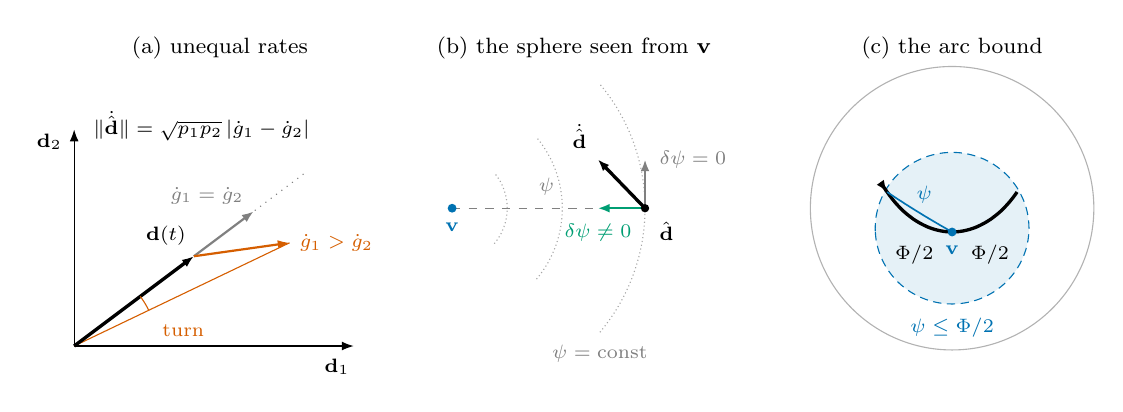
\begin{tikzpicture}[font=\scriptsize, >={Latex[length=1.5mm]},
  ttl/.style={font=\footnotesize, anchor=north}]
% (a) rotation from unequal logarithmic rates, d = 2
\node[ttl] at (1.85,4.05) {(a) unequal rates};
\draw[->] (0,0) -- (3.55,0) node[below left=1pt and -2pt] {$\dvec_1$};
\draw[->] (0,0) -- (0,2.75) node[below left=-2pt and 1pt] {$\dvec_2$};
\node[anchor=north west] at (0.12,3.1) {$\|\dot{\dhat}\|=\sqrt{p_1p_2}\,|\dot g_1-\dot g_2|$};
\draw[dotted, gray] (0,0) -- (2.964,2.223);
\draw[hired] (0,0) -- (2.736,1.311);
\draw[->, very thick] (0,0) -- (1.52,1.14) node[above left=0pt and -1pt] {$\dvec(t)$};
\draw[->, thick, gray] (1.52,1.14) -- (2.28,1.71) node[above left=-1pt and 0pt] {$\dot g_1=\dot g_2$};
\draw[->, thick, hired] (1.52,1.14) -- (2.736,1.311) node[right] {$\dot g_1>\dot g_2$};
\draw[hired] (25.602:1.05) arc[start angle=25.602, end angle=36.87, radius=1.05];
\node[hired, anchor=north west] at (0.997,0.394) {turn};
% (b) a sector of the sphere seen from v
\begin{scope}[shift={(6.35,1.75)}]
\node[ttl] at (0,2.3) {(b) the sphere seen from $\mathbf v$};
\draw[gray!70, densely dotted] (-1.014,-0.45) arc[start angle=-40, end angle=40, radius=0.7];
\draw[gray!70, densely dotted] (-0.478,-0.9) arc[start angle=-40, end angle=40, radius=1.4];
\draw[gray!70, densely dotted] (0.327,-1.575) arc[start angle=-40, end angle=40, radius=2.45];
\node[gray, anchor=north] at (0.327,-1.615) {$\psi=\mathrm{const}$};
\draw[dashed, gray] (-1.55,0) -- (0.3,0);
\node[gray, anchor=south] at (-0.35,0.04) {$\psi$};
\fill[hiblue] (-1.55,0) circle (1.6pt);
\node[hiblue, anchor=north] at (-1.55,-0.06) {$\mathbf v$};
\draw[->, thick, higreen] (0.9,0) -- (0.3,0);
\node[anchor=north east, higreen] at (0.85,-0.08) {$\delta\psi\neq0$};
\draw[->, thick, gray] (0.9,0) -- (0.9,0.62);
\node[anchor=west, gray] at (0.96,0.62) {$\delta\psi=0$};
\draw[->, very thick] (0.9,0) -- (0.3,0.62);
\node[anchor=south east] at (0.28,0.64) {$\dot{\dhat}$};
\fill (0.9,0) circle (1.5pt);
\node[anchor=north west] at (0.96,-0.05) {$\dhat$};
\end{scope}
% (c) the arc bound
\begin{scope}[shift={(11.15,1.75)}]
\node[ttl] at (0,2.3) {(c) the arc bound};
\draw[gray!60] (0,0) circle (1.8);
\fill[hiblue!10] plot[smooth cycle] coordinates {(-0.977,-0.253) (-0.975,-0.304) (-0.971,-0.354) (-0.965,-0.404) (-0.955,-0.454) (-0.943,-0.503) (-0.929,-0.551) (-0.912,-0.598) (-0.892,-0.645) (-0.87,-0.69) (-0.846,-0.735) (-0.819,-0.778) (-0.79,-0.819) (-0.759,-0.859) (-0.726,-0.897) (-0.691,-0.934) (-0.654,-0.969) (-0.615,-1.001) (-0.574,-1.032) (-0.532,-1.061) (-0.488,-1.087) (-0.444,-1.111) (-0.397,-1.133) (-0.35,-1.152) (-0.302,-1.169) (-0.253,-1.183) (-0.203,-1.195) (-0.153,-1.204) (-0.102,-1.211) (-0.051,-1.215) (0,-1.216) (0.051,-1.215) (0.102,-1.211) (0.152,-1.204) (0.203,-1.195) (0.252,-1.183) (0.301,-1.169) (0.35,-1.152) (0.397,-1.133) (0.443,-1.111) (0.488,-1.087) (0.531,-1.061) (0.573,-1.032) (0.614,-1.001) (0.653,-0.969) (0.69,-0.934) (0.725,-0.897) (0.758,-0.859) (0.789,-0.819) (0.818,-0.778) (0.845,-0.735) (0.869,-0.69) (0.891,-0.645) (0.911,-0.598) (0.928,-0.551) (0.943,-0.503) (0.955,-0.454) (0.964,-0.404) (0.971,-0.354) (0.975,-0.304) (0.976,-0.253) (0.975,-0.203) (0.97,-0.153) (0.964,-0.103) (0.955,-0.053) (0.943,-0.004) (0.928,0.044) (0.911,0.091) (0.891,0.138) (0.869,0.183) (0.845,0.228) (0.818,0.271) (0.789,0.312) (0.758,0.352) (0.725,0.391) (0.69,0.427) (0.653,0.462) (0.614,0.494) (0.573,0.525) (0.531,0.554) (0.488,0.58) (0.443,0.604) (0.397,0.626) (0.349,0.645) (0.301,0.662) (0.252,0.676) (0.203,0.688) (0.152,0.697) (0.102,0.704) (0.051,0.708) (0,0.709) (-0.052,0.708) (-0.102,0.704) (-0.153,0.697) (-0.203,0.688) (-0.253,0.676) (-0.302,0.662) (-0.35,0.645) (-0.397,0.626) (-0.444,0.604) (-0.489,0.58) (-0.532,0.554) (-0.574,0.525) (-0.615,0.494) (-0.654,0.462) (-0.691,0.427) (-0.726,0.391) (-0.759,0.352) (-0.79,0.312) (-0.819,0.271) (-0.846,0.228) (-0.87,0.183) (-0.892,0.138) (-0.912,0.091) (-0.929,0.044) (-0.943,-0.004) (-0.955,-0.053) (-0.965,-0.103) (-0.971,-0.153) (-0.975,-0.203)};
\draw[hiblue, densely dashed] plot[smooth cycle] coordinates {(-0.977,-0.253) (-0.975,-0.304) (-0.971,-0.354) (-0.965,-0.404) (-0.955,-0.454) (-0.943,-0.503) (-0.929,-0.551) (-0.912,-0.598) (-0.892,-0.645) (-0.87,-0.69) (-0.846,-0.735) (-0.819,-0.778) (-0.79,-0.819) (-0.759,-0.859) (-0.726,-0.897) (-0.691,-0.934) (-0.654,-0.969) (-0.615,-1.001) (-0.574,-1.032) (-0.532,-1.061) (-0.488,-1.087) (-0.444,-1.111) (-0.397,-1.133) (-0.35,-1.152) (-0.302,-1.169) (-0.253,-1.183) (-0.203,-1.195) (-0.153,-1.204) (-0.102,-1.211) (-0.051,-1.215) (0,-1.216) (0.051,-1.215) (0.102,-1.211) (0.152,-1.204) (0.203,-1.195) (0.252,-1.183) (0.301,-1.169) (0.35,-1.152) (0.397,-1.133) (0.443,-1.111) (0.488,-1.087) (0.531,-1.061) (0.573,-1.032) (0.614,-1.001) (0.653,-0.969) (0.69,-0.934) (0.725,-0.897) (0.758,-0.859) (0.789,-0.819) (0.818,-0.778) (0.845,-0.735) (0.869,-0.69) (0.891,-0.645) (0.911,-0.598) (0.928,-0.551) (0.943,-0.503) (0.955,-0.454) (0.964,-0.404) (0.971,-0.354) (0.975,-0.304) (0.976,-0.253) (0.975,-0.203) (0.97,-0.153) (0.964,-0.103) (0.955,-0.053) (0.943,-0.004) (0.928,0.044) (0.911,0.091) (0.891,0.138) (0.869,0.183) (0.845,0.228) (0.818,0.271) (0.789,0.312) (0.758,0.352) (0.725,0.391) (0.69,0.427) (0.653,0.462) (0.614,0.494) (0.573,0.525) (0.531,0.554) (0.488,0.58) (0.443,0.604) (0.397,0.626) (0.349,0.645) (0.301,0.662) (0.252,0.676) (0.203,0.688) (0.152,0.697) (0.102,0.704) (0.051,0.708) (0,0.709) (-0.052,0.708) (-0.102,0.704) (-0.153,0.697) (-0.203,0.688) (-0.253,0.676) (-0.302,0.662) (-0.35,0.645) (-0.397,0.626) (-0.444,0.604) (-0.489,0.58) (-0.532,0.554) (-0.574,0.525) (-0.615,0.494) (-0.654,0.462) (-0.691,0.427) (-0.726,0.391) (-0.759,0.352) (-0.79,0.312) (-0.819,0.271) (-0.846,0.228) (-0.87,0.183) (-0.892,0.138) (-0.912,0.091) (-0.929,0.044) (-0.943,-0.004) (-0.955,-0.053) (-0.965,-0.103) (-0.971,-0.153) (-0.975,-0.203)};
\draw[->, very thick] plot[smooth] coordinates {(0.825,0.206) (0.794,0.162) (0.761,0.119) (0.727,0.077) (0.691,0.037) (0.654,-0.002) (0.616,-0.039) (0.576,-0.074) (0.535,-0.106) (0.494,-0.137) (0.451,-0.165) (0.408,-0.19) (0.364,-0.213) (0.32,-0.234) (0.275,-0.252) (0.229,-0.267) (0.184,-0.279) (0.138,-0.289) (0.092,-0.296) (0.046,-0.3) (0,-0.302) (-0.046,-0.3) (-0.092,-0.296) (-0.138,-0.289) (-0.184,-0.279) (-0.229,-0.267) (-0.275,-0.252) (-0.32,-0.234) (-0.364,-0.213) (-0.408,-0.19) (-0.451,-0.165) (-0.494,-0.137) (-0.535,-0.106) (-0.576,-0.074) (-0.616,-0.039) (-0.654,-0.002) (-0.691,0.037) (-0.727,0.077) (-0.761,0.119) (-0.794,0.162) (-0.825,0.206) (-0.825,0.206)};
\draw[hiblue, semithick] plot[smooth] coordinates {(0,-0.302) (-0.023,-0.289) (-0.045,-0.277) (-0.067,-0.264) (-0.089,-0.251) (-0.112,-0.238) (-0.134,-0.226) (-0.156,-0.213) (-0.178,-0.2) (-0.2,-0.187) (-0.222,-0.174) (-0.244,-0.161) (-0.266,-0.148) (-0.288,-0.135) (-0.31,-0.122) (-0.332,-0.109) (-0.354,-0.096) (-0.375,-0.083) (-0.397,-0.069) (-0.418,-0.056) (-0.44,-0.043) (-0.461,-0.03) (-0.482,-0.017) (-0.504,-0.003) (-0.525,0.01) (-0.545,0.023) (-0.566,0.036) (-0.587,0.049) (-0.608,0.063) (-0.628,0.076) (-0.648,0.089) (-0.669,0.102) (-0.689,0.115) (-0.709,0.128) (-0.728,0.141) (-0.748,0.154) (-0.767,0.167) (-0.787,0.18) (-0.806,0.193) (-0.825,0.206)};
\node[hiblue, anchor=south] at (-0.354,-0.056) {$\psi$};
\fill[hiblue] (0,-0.302) circle (1.6pt);
\node[hiblue, anchor=north] at (0,-0.352) {$\mathbf v$};
\node[anchor=north] at (0.48,-0.346) {$\Phi/2$};
\node[anchor=north] at (-0.481,-0.345) {$\Phi/2$};
\node[hiblue, anchor=north] at (0,-1.266) {$\psi\le\Phi/2$};
\end{scope}
\end{tikzpicture}
\caption{Mechanism of the rotation and of the arc bound. (a)~The signal vector $\dvec$ of \eqref{eq:dvec} for $d=2$: when both components grow at the same logarithmic rate the direction $\dhat$ is unchanged, and it turns only when the rates differ, at the speed \eqref{eq:repl}. (b)~A sector of the unit sphere seen from $\mathbf v$: the sets of constant $\psi$, and hence of constant loss, are circles around $\mathbf v$, and the great circles through $\mathbf v$ are radial lines. Only the component of $\dot{\dhat}$ along the great circle through $\mathbf v$ changes $\psi$ ($\delta\psi\neq0$); the other $d-2$ components move $\dhat$ within its level set ($\delta\psi=0$). (c)~A path of $\dhat$ of length $\Phi$, split at its midpoint into two halves of length $\Phi/2$. Every point of the path lies within $\Phi/2$ of the midpoint along the path, and therefore on the sphere, so an indicator $\mathbf v$ at the midpoint keeps $\psi\le\Phi/2$ (shaded cap), which gives \eqref{eq:arcbound}. Panels (b) and (c) hold in any dimension and are drawn for $d=3$.}
\label{fig:arcmech}
\end{figure*}
%</mechfig:arc>

\subsection{A bound in terms of the rotation arc}

Suppose that over a window of the service life the informative direction
traverses a path of total length $\Phi<\pi$ on the sphere, called its arc.
The direction at the midpoint of this arc lies within $\Phi/2$ of every point
on it (Fig.~\ref{fig:arcmech}(c)), so a fixed indicator placed at the midpoint satisfies $\psi\le\Phi/2$
throughout. Since the loss increases with $\psi$, such an indicator
satisfies, at every instant,
\begin{equation}
e^{2\lloss}\le\frac{1}{1-w\sin^{2}(\Phi/2)}\le\frac{1}{\cos^{2}(\Phi/2)} .
\label{eq:arcbound}
\end{equation}
The same holds for any fixed indicator whose largest angle to the path,
$\psi_{\max}$, is at most $\Phi/2$. The bound requires only the arc, which
can be estimated from run-to-failure data before any indicator is designed.
An arc of $30^{\circ}$ allows at most $7.2\%$ additional error variance,
$60^{\circ}$ at most $33\%$, and $90^{\circ}$ a doubling; the right-hand
bound corresponds to the limit of high signal-to-noise ratio and is
independent of $\gamma$. Correspondingly, the safety margin of the
replacement policy of Section~\ref{sec:loss} grows by at most the factor
$1/\cos(\Phi/2)$. The best fixed indicator lies close to the midpoint of the
arc; Supplementary Section~S2 characterises it as a barycentre of the path
of the informative direction. Figure~\ref{fig:mech}(a) shows how the loss
grows with the misalignment angle, and Fig.~\ref{fig:mech}(b) the rotation
measured on the battery cells of Section~\ref{sec:cells}.

\begin{figure}[t]
\centering 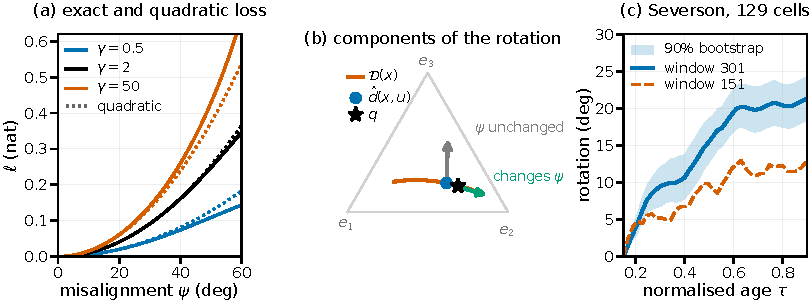
\includegraphics{fig2.pdf}
\caption{(a)~The exact loss \eqref{eq:exact} (solid) and its quadratic approximation (dotted); the approximation overstates the loss when $\gamma<2$ and understates it when $\gamma>2$. (b)~Rotation of the observed direction on the Severson battery cells (Section~\ref{sec:cells}), estimated with smoothing windows of $301$ and $151$ cycles.}
\label{fig:mech}
\end{figure}

\subsection{Design procedure}
\label{sec:procedure}

The bound yields a design procedure that requires run-to-failure data only.
\begin{enumerate}
\item Estimate the informative direction from the fleet: at each value of the
normalised life $\tau$, take the time derivative of the monitoring channels,
whiten each channel by its measurement noise, estimated from the scatter of
the channel about a smoothed trend, and average the resulting unit vectors
over the units. The result is called the observed direction.
\item Compute the arc $\Phi$ that the observed direction traverses and the
bound \eqref{eq:arcbound}. The bound is the largest increase in error variance
that a well-placed fixed indicator can cause; if it is small compared with
the accuracy the maintenance decision requires, a fixed indicator suffices.
\item Place the fixed indicator at the barycentre of the path, in practice
the renormalised mean of the observed direction, and check that its largest
angle to the path does not exceed $\Phi/2$.
\item Validate the indicator with a leave-one-out remaining-life estimator,
against the same estimator run on all channels.
\item Evaluate the maintenance decision that the estimate supports.
\end{enumerate}
Section~\ref{sec:cells} carries out the five steps on measured lithium-ion
cells.

\section{Case study: lithium-ion cells}
\label{sec:cells}

The procedure is applied to the lithium-ion cells of Severson et
al.~\cite{severson2019}, a public fleet cycled to failure under different
fast-charging protocols and widely used as a prognostics benchmark. The
monitoring channels are discharge capacity, internal resistance and mean cell
temperature. The $129$ cells that meet the selection
criteria of the protocol in Supplementary Section~S1 have lives from $447$ to $1932$ cycles;
because the lives differ more than fourfold across protocols, the population
is far from a time shift. The cells therefore violate (A1), and the
procedure treats them as if they differed only in age along a common path in
normalised life; the leave-one-out test of step 4 checks whether that
approximation is good enough in practice. (A3) and (A4) are not needed here.
Supplementary Section~S1 gives the protocol and parameters of every step.

\subsection{Steps 1 to 3: rotation, bound and indicator}

The observed direction of step~1, which estimates the informative direction
as a fleet mean, moves through an arc of $30.7^{\circ}$
between $15\%$ and $90\%$ of life (Fig.~\ref{fig:mech}(b)). After whitening,
the fixed indicator at its barycentre weights capacity, resistance and
temperature as $(0.99,0.10,0.12)$ and lies at most $14^{\circ}$ from the
informative direction, within half the arc. By \eqref{eq:arcbound}, it
therefore inflates the error variance of the remaining-life estimate by at
most $7.5\%$ over that window, irrespective of the signal-to-noise ratio, and
widens the safety margin of a predictive replacement policy by at most
$3.7\%$.

\subsection{Step 4: remaining-life estimation}

The bound concerns the optimal estimate given the record at one inspection.
A practical estimator uses a history of inspections and is not optimal, so
its error with the fixed indicator can fall on either side of its error with
all channels; what the comparison tests is whether the information loss
matters for such an estimator. A similarity-based estimator matches the last
$30\%$ of a cell's elapsed cycles against the fleet reference path in
normalised life and returns the life that fits best; everything it uses,
including the fixed indicator, is computed without the cell being tested.
With all three channels its root-mean-square error is $148$, $83$ and $49$
cycles at $50\%$, $70\%$ and $90\%$ of life. Run on the fixed indicator at
the barycentre of the observed direction, the same estimator attains between
$0.96$ and $1.00$ times the mean squared error of the three-channel estimator
at these ages (Table~\ref{tab:cells}). Capacity alone, the conventional
battery health indicator, lies up to $22^{\circ}$ from the informative
direction, for which the bound allows $17\%$, and raises the mean squared
error by $5\%$ at half of life and by less later. Temperature alone, a
deliberately misaligned control, raises it at least $40$-fold, so the test is
able to detect a poorly chosen indicator. A data-level fusion indicator,
whose weights minimise the between-cell spread of the indicator at failure
relative to its mean change over life, in the spirit of~\cite{liu2013fusion},
lies $75^{\circ}$ to $82^{\circ}$ from the informative direction and has
$28.9$ times the mean squared error at half of life. Near failure, the stage
its construction targets, it is the most accurate signal, at $0.81$ times the
three-channel error: it suppresses between-cell differences in the level of
the channels at failure, a source of error that a time-shift population does
not contain.

\begin{table*}[t]
\caption{Case study on the Severson cells. $\psi_{\max}$ is the largest angle between the estimator input and the fleet-mean informative direction over $\tau\in[0.15,0.90]$; the mean-squared-error (MSE) ratios compare the leave-one-out remaining-life estimator run on the input with the same estimator run on all three channels, at $50\%$, $70\%$ and $90\%$ of life; the replacement columns give the minimal long-run cost per $1000$ cycles, in units of a preventive replacement, when a failure costs ten times as much, with the fraction of cells failing and the mean life left unused at replacement, in cycles.}
\label{tab:cells}
\centering
\small
\setlength{\tabcolsep}{4pt}
\begin{tabular}{lccccccc}
\hline
 & & \multicolumn{3}{c}{MSE ratio} & \multicolumn{3}{c}{replacement policy} \\
estimator input & $\psi_{\max}$ & $50\%$ & $70\%$ & $90\%$ & cost & failures & unused\\
\hline
all channels & --- & $1$ & $1$ & $1$ & $1.689$ & $1.6\%$ & $134$\\
fixed indicator & $14^{\circ}$ & $0.960$ & $0.972$ & $0.999$ & $1.688$ & $1.6\%$ & $133$\\
capacity & $22^{\circ}$ & $1.050$ & $1.014$ & $0.986$ & $1.690$ & $1.6\%$ & $134$\\
fusion & $82^{\circ}$ & $28.9$ & $8.43$ & $0.807$ & $1.731$ & $1.6\%$ & $150$\\
temperature & $90^{\circ}$ & $43.7$ & $171$ & $725$ & --- & --- & ---\\
\hline
\end{tabular}
\end{table*}

\subsection{Step 5: replacement decisions}

The last step evaluates the decision directly. Each cell is inspected every
$25$ cycles from cycle $100$ and is replaced at the first inspection at which
the predicted remaining life is at most a threshold of $n_{\mathrm{thr}}$
cycles; a cell not replaced before its end of life counts as a failure. For a
failure ten times as costly as a preventive replacement, the threshold that
minimises the long-run cost per cycle~\cite{kamariotis2024metric} gives the
costs of Table~\ref{tab:cells}. The fixed indicator, capacity alone and all three
channels reach the same cost to within $0.1\%$, with $1.6\%$ of cells
failing and about $134$ cycles, a fifth of a cell's life, left unused at
replacement; the fusion indicator costs $2.5\%$ more. For cost ratios from
$5$ to $50$ the fixed indicator stays within $1\%$ of the three-channel
cost. The thresholds are chosen on the same cells for every input, so the
absolute costs are optimistic, but the comparison between inputs is not. The
case study thus confirms, on measured data and at the level of a maintenance
decision, what the bound predicts: for this fleet a fixed indicator is
adequate.

\section{Selecting the operating point}
\label{sec:steer}

The case study took the operating conditions as given. In many applications
they are not: operators choose temperatures, loads or charging rates, often
to extend life. Because the operating point sets the relative rates of the
mechanisms, it also moves the informative direction, and it could in
principle be chosen to keep a fixed indicator aligned. This practice,
referred to here as steering, is examined in this section. No public fleet
lets the operating point act on the damage (Section~\ref{sec:data}), so the
examination uses a synthetic system. Section~\ref{sec:arc} already limits
what steering can achieve: the excess error variance that it can remove is
at most the bound \eqref{eq:arcbound} for the arc of the unsteered
trajectory.

\subsection{Limits of steering}
\label{sec:limit}

At a state $x$, the directions attainable through the operating point form
the set
\begin{equation}
\mathcal D(x)=\{\dhat(x,u):u\in\mathcal U\},
\label{eq:reachset}
\end{equation}
and the smallest misalignment achievable at $x$, called the floor, is
$\beta_{\min}(x)=\angle(\mathbf v,\mathcal D(x))$. Two structural
results, derived in Supplementary Section~S4, delimit what steering can do.
First, holding the
misalignment at a constant, non-zero level is a single scalar condition and
needs only one adjustable operating variable. Second, removing the loss
altogether is far more demanding. If the informative direction equals
$\mathbf v$ at every instant, the damage can only grow along the fixed
direction $\Sigma^{1/2}\mathbf v$, so the state must move along a straight
line in damage space. Keeping it on that line requires, except for special
combinations of parameters, one fewer independent operating variable than
there are mechanisms, together with an aligning input that stays within the
allowed envelope $\mathcal U$ along the whole line. A component with three
mechanisms and a single temperature setpoint can therefore reduce the loss
but, generically, not remove it.

When the loss cannot be removed, the relevant quantity is the smallest
achievable average loss,
\begin{equation}
\bar\lloss^{\star}=\min_{u(\cdot)}\frac{1}{T_f}\int_{0}^{T_f}\lloss\,dt ,
\label{eq:frac}
\end{equation}
over all operating policies $u(\cdot)$, that is, all ways of setting the
operating point over time. Both the integral and the lifetime $T_f$ depend
on the policy, so the objective is a ratio of two quantities that the
operating point changes together, and the operating point that aligns the
indicator is in general not the one that prolongs life. The simplest
policy disregards the lifetime and applies, at each state, the input that
minimises the misalignment; it is referred to as the myopic policy.

\subsection{A numerical study}
\label{sec:case}
\label{sec:testplant}

The synthetic system is chosen to resemble the thermally activated
degradation of a battery with three mechanisms and one adjustable
temperature. It has $d=3$ mechanisms with Arrhenius factors
$\varphi_i(u)=e^{\theta_i-E_iu}$, in which the input $u$ is a scaled
reciprocal temperature, $u=3\,(1/(kT)-1/(kT_{60}))/(1/(kT_{25})-1/(kT_{60}))$
with $T_{60}$ and $T_{25}$ the absolute temperatures of $60$ and
$25\,^{\circ}$C, so that $u=0$ corresponds to $60\,^{\circ}$C and $u=3$ to
$25\,^{\circ}$C. The parameters are $\theta=(0,0.3,-0.2)$ and
$E=(0.6,1.1,0.8)$, which in these units are activation energies of $0.44$,
$0.81$ and $0.59$~eV, with shape functions $h_i(x)=1+c_ix$ and
$c=(-0.5,2.0,0.8)$, which give one decelerating and two accelerating
mechanisms. Time is measured in units of the characteristic time of the
first mechanism at $60\,^{\circ}$C, where $\varphi_1=1$. There is a single
input $u\in[0,3]$, so by Section~\ref{sec:limit} the loss can be reduced but,
generically, not removed; Supplementary Section~S4 confirms this for the
present system. The noise has unit variance and the prior variance is
$\Var[R]=10^{3}$; the weight $w=\gamma/(1+\gamma)$ of \eqref{eq:exact} is evaluated at the system's own $\gamma=\|\dvec\|^{2}\Var[R]$ at each state rather than held fixed. Every trajectory starts from $x_i(0)=5\times10^{-3}$ and runs to the condemnation limit $x_f=0.9$; the values of the reported constants at $x_f=1$ are given in Supplementary Section~S4. The identities of Sections~\ref{sec:model} and~\ref{sec:arc} were verified numerically on this system (Supplementary Section~S3).

The bound of Section~\ref{sec:arc} can be checked first. Under constant
inputs the arc is between
$24.8^{\circ}$ and $35.6^{\circ}$, the bound allows between $4.8\%$ and
$10.3\%$, and the best fixed indicator for each input incurs between $1.6\%$
and $3.4\%$; the bound therefore holds and overestimates the excess by a
factor of about three. These small excesses are all that steering can remove.

The comparison of strategies needs three indicators. The steering indicator
$q^{\star}$ is the one for which the myopic policy achieves the smallest
average loss; the balanced indicator weights the three whitened channels
equally; and for each constant operating point, the constant design uses the
indicator that is best for that point. With the input of the myopic policy
searched on a grid of $41$ points of $\mathcal U$, the steering indicator has
the weight vector
$\mathbf v^{\star}=(0.466,0.771,0.435)$, at which the myopic policy attains
$1.68\times10^{-4}$ against $1.15\times10^{-2}$ under the best constant input, a factor of $68$. This comparison holds the indicator fixed at the one
designed for steering. For operation without steering, the indicator would
instead be designed for the constant input, and minimising over the indicator
and the constant input jointly gives $7.95\times10^{-3}$, at the
high-temperature end $u=0$ of the envelope. Relative to this baseline, the
reduction achieved by steering is a factor of $47$, the figure quoted in the
abstract. The myopic policy is also close to the best achievable by any
policy: the best policy for the ratio \eqref{eq:frac}, computed on state grids of
up to $137$ points per axis, lies within $2.1\%$ of it on every control grid,
and both factors are stable under refinement of the grids (Supplementary
Section~S4).

Table~\ref{tab:policy} reports the practical consequences. By
\eqref{eq:mmse}, a loss of $7.95\times10^{-3}$ already corresponds to an
error variance only $1.6\%$ above that of the complete record, and steering
removes almost all of this excess. A practical estimator, however, is largely
insensitive to it. A time-shifted population is simulated along the path of
each policy, each unit is observed at $30$ instants over the last $40\%$ of
a lifetime before its remaining life is estimated, with unit channel noise,
and the estimate is the time offset that best matches the reference path of
the policy, computed once from the indicator and once from all three
channels. Under every policy the two estimators
differ by less than $1.2\%$, and the error as a fraction of life stays between
$8.4\%$ and $10.7\%$, being determined by the path rather than by the
indicator. The operating point does, however, change the lifetime
substantially. Across the constant designs of the table it varies $19$-fold,
because the mechanisms run faster when hot. Among the policies, the myopic
policy at $q^{\star}$ attains a lifetime $1.66$ times that of the best
constant input at the same indicator and $3.8$ times that of the constant
design with the smallest loss; and a myopic policy aimed at the balanced
indicator, which requires far less steering, extends the lifetime by a
further factor of $3.4$. For this system the choice of operating point
matters far more for lifetime than for monitoring.

\begin{table*}[t]
\caption{Information loss, remaining-life estimation error and lifetime of the synthetic system under different operating strategies. $\bar\lloss$ is the information loss \eqref{eq:objective}; $e^{2\bar\lloss}-1$ the corresponding excess error variance \eqref{eq:mmse}; the remaining-useful-life (RUL) errors are the median absolute error of a
template-matching remaining-life estimator over $2000$ units, as a percentage of life, based on the indicator or on all three channels; $T_f$ is the lifetime. Constant designs use the indicator that is best for their own input.}
\label{tab:policy}
\centering
\small
\begin{tabular}{lccccc}
\hline
 & & & \multicolumn{2}{c}{RUL error (\% of life)} & \\
operating strategy & $\bar\lloss$ & $e^{2\bar\lloss}-1$ & indicator & all channels & $T_f$\\
\hline
constant, $60\,^{\circ}$C & $7.95\times10^{-3}$ & $1.6\%$ & $10.7\%$ & $10.8\%$ & $0.378$\\
constant, $41.5\,^{\circ}$C & $1.44\times10^{-2}$ & $2.9\%$ & $8.9\%$ & $8.8\%$ & $1.967$\\
constant, $25\,^{\circ}$C & $1.26\times10^{-2}$ & $2.6\%$ & $8.8\%$ & $8.7\%$ & $7.203$\\
myopic, $q^{\star}$ & $1.68\times10^{-4}$ & $0.03\%$ & $9.5\%$ & $9.5\%$ & $1.433$\\
myopic, balanced & $4.08\times10^{-3}$ & $0.8\%$ & $8.4\%$ & $8.5\%$ & $4.928$\\
\hline
\end{tabular}
\end{table*}

\subsection{Sensitivity to model misspecification}
\label{sec:misspec}

Where run-to-failure data are scarce, the indicator can instead be designed
from a degradation model, by applying steps 1 to 3 of the procedure to
trajectories simulated from the model. Such an indicator inherits the errors
of the model, and this subsection asks how accurate the model must be. For
each error level $\omega$, a perturbed energy vector $E(1+\omega\eta)$ is
drawn, with $\eta$ standard normal, and the barycentre indicator is computed
from trajectories of this misspecified system under a constant input. The
indicator is then evaluated on the true system under the myopic policy aimed
at it, with every loss evaluated at the system's own $\gamma$. Since the
policy is computed from the true system, the table isolates the effect of an
error in the indicator; an error that also affected the policy would be more
costly. Table~\ref{tab:misspec} reports the loss ratio, the loss of this
indicator divided by that of the indicator designed from the true model, over
$40$ draws per level; a ratio of $1$ indicates that the error has no effect.

\begin{table}[t]
\caption{Effect of designing the indicator from a misspecified stress model.
Entries are the loss ratio: the loss on the true system relative to that of
the indicator designed from the true model, over $40$ draws per level;
$\omega$ is the relative standard deviation of the error in the activation
energies. The steering policy uses the true system.}
\label{tab:misspec}
\centering
\begin{tabular}{cccc}
\hline
$\omega$ & median & 90th percentile & worst of $40$\\
\hline
$0.02$ & $1.03$ & $1.52$ & $2.04$\\
$0.05$ & $1.40$ & $2.94$ & $6.44$\\
$0.10$ & $3.10$ & $10.8$ & $67.7$\\
$0.20$ & $10.0$ & $44.9$ & $78.6$\\
$0.35$ & $36.0$ & $94.1$ & $195$\\
\hline
\end{tabular}
\end{table}

An error of $2\%$ in the energies has a negligible effect. At $5\%$ the
median loss ratio is $1.40$. At $10\%$ the median loss ratio is $3.10$ and
the worst of forty draws reaches $67.7$, comparable in magnitude to the entire
benefit of steering; beyond this level every column increases monotonically,
to a median of $36.0$ at $\omega=0.35$. The loss to which these ratios apply
is small, however, so that even a tenfold increase leaves the indicator's
excess error variance below $1\%$.

\section{Evidence from public run-to-failure data}
\label{sec:data}

The preceding sections rest on premises that public run-to-failure data can
partly test. Three are examined here: that the informative direction rotates; that the operating point moves it by
acting on the degradation, the actuation premise on which
Section~\ref{sec:steer} relies; and that the separable stress model (A4),
interpreted through the pairing of channels with mechanisms (A3), holds.
The tests use the observed direction of step 1 of the procedure, estimated
from data, which coincides with the informative direction only under (A1)
and (A3).
Table~\ref{tab:fleets} summarises what six public run-to-failure fleets establish and what they leave open. The fleets are the Severson battery cells, the XJTU-SY and PRONOSTIA bearing test rigs, the NASA battery cells, and the C-MAPSS and N-CMAPSS turbofan engine simulations of NASA. Supplementary Section~S1 gives the
protocol behind every row, and its Table~S1 lists the parameters of the code
that produced it.

\begin{table*}[tb]
\caption{Premises of the model examined on six public run-to-failure fleets.
Only the two turbofan simulations vary the operating point within a unit, and
neither allows it to act on the damage; the actuation premise is therefore
untested on every public fleet. $B$ and $W$ are the mean angles between observed directions of different operating regimes and of two halves of the same regime.}
\label{tab:fleets}
\centering
\footnotesize
\setlength{\tabcolsep}{3pt}
\begin{tabular}{@{}R{0.16}R{0.14}R{0.31}R{0.34}@{}}
\hline
fleet & premise & quantity measured & finding\\
\hline
Severson lithium-ion~\cite{severson2019} & rotation &
arc of an empirically constructed informative direction, the fleet mean, over $\tau\in[0.15,0.9]$, on
$129$ Severson lithium-ion cells &
travels $30.7^{\circ}$ of arc and ends $21^{\circ}$ from its start
(Fig.~\ref{fig:mech}(b)); all three weights stay positive once the
smoothing window reaches $301$ cycles\\[3pt]
XJTU-SY~\cite{xjtu2020}, PRONOSTIA~\cite{pronostia2012} & actuation &
--- & the operating condition is fixed per unit, so condition and group of
units cannot be separated\\[3pt]
NASA batteries~\cite{saha2007} & actuation & --- & only four cells\\[3pt]
C-MAPSS~\cite{saxena2008} & actuation: not testable &
between-regime minus within-regime angle, $B-W$, each engine serving as its own
control &
by $7.9^{\circ}$ (FD004) and $10.8^{\circ}$ (FD002), positive for $436$ of $439$ engines; surrogate regimes give $\lvert B-W\rvert\le0.5^{\circ}$; the damage is independent of the regime by construction, so the contrast reflects the sensor map\\[3pt]
N-CMAPSS DS02, DS01~\cite{arias2021} & separability with pairing~\eqref{eq:obs} &
interaction against both main effects, in a two-way layout inside engines &
larger by a factor $1.65$ over the operating-point effect on DS02 and $1.84$ on DS01, under every clustering and staging tried: \textbf{rejected} jointly\\
\hline
\end{tabular}
\end{table*}

Rotation of the informative direction is observed on the battery cells of
Section~\ref{sec:cells}. That analysis and the turbofan contrasts below
interpret a time derivative as the sensitivity \eqref{eq:sens}, and
therefore presuppose the time-shift population (A1).

The effect of the operating point on degradation remains untested. The
measured fleets either do not vary the operating point within a unit or
contain too few units. The two turbofan simulations do vary it, between
discrete operating regimes of altitude, speed and throttle, but their
generators preclude the test. C-MAPSS imposes its flow and efficiency losses
as exponential functions of time, from a random initial deterioration, and
lets the regime act only on the thermodynamic response of the
sensors~\cite{saxena2008}. N-CMAPSS imposes a linear normal degradation
followed by a steeper abnormal one, with the operating history entering
through the onset of the abnormal phase~\cite{arias2022fusing}, and the health
parameters supplied with the data are constant within every flight. On
C-MAPSS the observed directions of different regimes of the same engine
differ by more ($B$) than those of two halves of one regime ($W$). This
contrast, positive in all but three engines against a negative
control that returns none, therefore shows that the observed direction
depends on the regime through the sensor response alone. Variable operating
conditions thus rotate the observed direction even when they do not act on
the damage. Because the loss of a fixed indicator depends on the observed
direction regardless of the cause of its motion, this finding is relevant to
indicator design; it is not, however, evidence that the operating point acts
on the damage.

The separable model fails on raw turbofan sensors. On both N-CMAPSS datasets
the interaction between operating point and life stage exceeds the main
effect of the operating point. The test rejects (A3) and (A4) jointly, and
since the simulated damage does not respond to the operating point within a
flight, the violation is attributable to the sensor map: the sensors mix
mechanisms with weights that depend on the operating point, in violation of
\eqref{eq:obs}. The pairing is
what makes the informative direction positive, so the geometry of
Sections~\ref{sec:arc} and~\ref{sec:steer} applies to such sensors only after
the observation map has been inverted, and the offline screen of how far
the operating point can move the informative direction (its actuation
authority; Supplementary Section~S4) is available only where the separable
form has been shown to hold. The two-way layout, whose
protocol is given in Supplementary Section~S1, provides this test at the cost
of a single pass over data that a reliability programme typically already
holds.

\section{Discussion and conclusions}
\label{sec:discussion}

The paper asked how much information about remaining life a fixed health
indicator discards when degradation mechanisms progress at different rates,
and whether the operating point can reduce the loss. The loss is set by how
far the informative direction turns over the life, and on the battery cells
examined here the turn is small enough that a fixed indicator supports
remaining-life estimates and replacement decisions as well as all channels
do. The operating point can reduce the loss, but when the turn is small there
is little to gain.

The results have three practical implications.

First, the rotation arc should be assessed before an adaptive indicator is
considered. The bound \eqref{eq:arcbound} converts a measured arc into a
worst-case increase in the error variance of the remaining-life estimate.
For the battery fleet examined here the resulting increase is at
most $7.5\%$, and for the synthetic system the actual excess is about one
third of the bound. Where
the arc amounts to a few tens of degrees, a single fixed indicator is
adequate; indicators whose weights change with age, whether adaptive,
segmented by life stage or learned, become worthwhile as the arc approaches a
right angle, at which the bound allows the error variance to double. The five
steps of Section~\ref{sec:procedure} make this assessment from run-to-failure
data alone.

Second, the operating point should be selected primarily for service life.
Steering the operating point can reduce the information loss by an order of
magnitude or more. Where the loss is already small, however, this yields
almost no improvement in the accuracy of a practical remaining-life
estimator, whereas the same choice alters the lifetime by an order of
magnitude. Aligning an indicator and prolonging the life of the component are
distinct objectives, and when the arc is small the latter is the more
consequential.

Third, variable operating conditions should be represented when the arc is
estimated. On the turbofan simulations the observed direction differs between
operating regimes even though the damage does not respond to them, because
the sensors respond differently in different regimes. An arc estimated under
a single operating condition can therefore understate the rotation that a
fixed indicator will meet in service.

\paragraph{Limitations} Four limitations qualify these conclusions. First,
the construction assumes a time-shift population (A1); dispersing the
degradation coefficients of the synthetic system rotates the population
regression of damage on remaining life by about $45^{\circ}$ away from the
direction the construction uses, more than the measured arc of the battery
cells, so the bound does not cover such dispersion, although the battery case
study, whose cells violate (A1), suggests that the practical conclusion
survives it.
Second, the pairing of channels with mechanisms (A3) fails on raw turbofan
sensors, so the geometry applies to them only after the observation map has
been inverted. Third, the actuation premise remains untested on every public
fleet. Finally, the best achievable loss is computed and bracketed between
the myopic policy and an extrapolation of the computation to infinitely fine
grids, not bounded analytically.

\appendix

\section{Derivations}
\label{app:derivations}

\subsection{Information loss and error-variance inflation}
\label{app:loss}
Write $\tilde y=\dvec R+\epsilon$ with $\epsilon\sim N(0,I_d)$, the
linearised whitened record. The indicator returns
$z=(\mathbf v^{\top}\dvec)R+\mathbf v^{\top}\epsilon$, whose noise is standard
normal because $\|\mathbf v\|=1$, so its signal-to-noise ratio is
$\gamma\cos^{2}\psi$. The record's sufficient statistic $\dvec^{\top}\tilde y$
has ratio $\gamma$. A scalar Gaussian channel of signal-to-noise ratio $s$
carries $\tfrac12\log(1+s)$ nats about $R$~\cite{cover2006}, so the loss,
the mutual information of $R$ with the record minus that with the indicator,
is the first form of \eqref{eq:exact}; substituting
$\cos^{2}\psi=1-\sin^{2}\psi$ gives the second. The posterior variances are
$\Var[R]/(1+\gamma\cos^{2}\psi)$ and $\Var[R]/(1+\gamma)$, whose quotient is
\eqref{eq:mmse}. Equation~\eqref{eq:fisherpair} is \eqref{eq:exact} with
$\gamma=\Var[R]I_{\mathrm{rec}}$ and $\gamma\cos^{2}\psi=\Var[R]I_z$; at fixed
$I_{\mathrm{rec}}$, $w$ is fixed and $\lloss$ increases continuously from zero
towards $\tfrac12\log(1+\gamma)$ as $\psi$ goes from $0$ to $\pi/2$.

\subsection{Rotation of the informative direction}
\label{app:rotation}
From $\dvec_i=e^{g_i}$, $\dot\dvec_i=\dvec_i\dot g_i$, and
$\dot{\dhat}=\|\dvec\|^{-1}(\dot\dvec-\dhat(\dhat^{\top}\dot\dvec))$ has
components $\dhat_i(\dot g_i-\E_p[\dot g])$ with $p_i=\dhat_i^{2}$, so its
squared norm is $\Var_p[\dot g]$. Differentiating
$g_i=\log\varphi_i(u)+\log h_i(x_i)-\log\sigma_i$ along \eqref{eq:plant}
gives $\dot g_i$ in \eqref{eq:repl}. With $\cos\psi=\dhat^{\top}\mathbf v$,
$-\sin\psi\,\dot\psi=\dot{\dhat}^{\top}\mathbf v$, so only the component of
$\dot{\dhat}$ along the great circle towards $\mathbf v$ changes $\psi$.

\section*{Data availability and reproducibility}
The six fleets named in Section~\ref{sec:data} are publicly available. One
script recomputes every reported number from a single configuration and
compares it with the value stated in this manuscript and in its
supplementary material, covering the tables and the quantities reported
alongside them; all of its checks pass, and the output of the run that
verified this version is included. The random-system sweep and the
downstream repetition of Supplementary Section~S4 and the grid sequence of
Section~\ref{sec:case} require several hours of computation, so they are
recorded by three further scripts; the checks read these records and
recompute part of the grid sequence afresh. One group of numbers lies
outside the checks: the residuals of the identity checks in Supplementary
Section~S3. The figures are produced by three further scripts. All of these
are available at
\url{https://github.com/HuyHoangLe0201/health-indicator-information-loss},
and are also provided with this article as a supplementary archive, together
with the Supplementary Material.

\section*{CRediT authorship contribution statement}
\textbf{Huy Hoang Le:} Conceptualization, Methodology, Formal analysis,
Software, Validation, Investigation, Data curation, Visualization,
Writing -- original draft. \textbf{Kim-Anh Nguyen:} Conceptualization,
Methodology, Validation, Writing -- review \& editing, Supervision, Project
administration.

\section*{Declaration of generative AI and AI-assisted technologies in the manuscript preparation process}
During the preparation of this work the authors used Claude (Anthropic) to
assist with drafting and editing the text and with writing and checking the
analysis and verification code. After using this tool, the authors reviewed
and edited the content as needed and take full responsibility for the content
of the published article.

\section*{Declaration of competing interest}
The authors declare that they have no known competing financial interests or personal relationships that could have appeared to influence the work reported in this paper.

\section*{Funding}
This research did not receive any specific grant from funding agencies in the public, commercial, or not-for-profit sectors.

\bibliographystyle{elsarticle-num} \bibliography{Ref}

\end{document}
